\section{Systemmodelle}

\subsection{Objektmodelle}
% UML Klassendiagramme

\begin{figure}[H]
\centering
\includegraphics[scale=0.5]{../system_models/object_models/lambda_calculus.pdf}
\caption{UML Klassendiagramm zum Lambda-Kalkül}
\end{figure}

\subsection{Dynamische Modelle}
% UML Zustandsautomat, Sequenzdiagramm

%\newgeometry{left=40pt}
\begin{figure}[H]
\centering
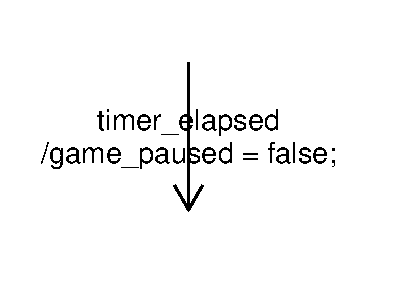
\includegraphics[scale=0.4]{../system_models/dynamic_models/menu_state_machine.pdf}
\caption{Zustandsautomat zur Menübedienung}
\end{figure}
%\restoregeometry

\begin{figure}[H]
\centering
\includegraphics[scale=0.55]{../system_models/dynamic_models/game_level_state_machine.pdf}
\caption{Zustandsautomat zum Ablauf eines Levels}
\end{figure}

\begin{figure}[H]
\centering
\includegraphics[scale=0.55]{../system_models/dynamic_models/reduction_mode_state_machine.pdf}
\caption{Zustandsautomat zur Funktion des Reduktions-Modus}
\end{figure}

%GUI

\subsection{Benutzerschnittstelle}

\begin{figure}[H]
\centering
\includegraphics[scale=0.55]{../gui/_jpeg_numeration/registration1.jpg}
\caption{Sprachauswahlmenü}
\label{fig:Sprachauswahlmenu}
\end{figure}

\begin{figure}[H]
\centering
\includegraphics[scale=0.55]{../gui/_jpeg_numeration/registration2.jpg}
\caption{Namenswahlmenü}
\label{fig:Namenswahlmenu}
\end{figure}

\begin{figure}[H]
\centering
\includegraphics[scale=0.55]{../gui/_jpeg_numeration/registration3.jpg}
\caption{Avatarauswahlmenü}
\label{fig:Avatarauswahlmenu}
\end{figure}

\begin{figure}[H]
\centering
\includegraphics[scale=0.55]{../gui/_jpeg_numeration/choose_profile.jpg}
\caption{Profilauswahlmenü}
\label{fig:Profilauswahlmenu}
\end{figure}

\begin{figure}[H]
\centering
\includegraphics[scale=0.55]{../gui/_jpeg_numeration/welcome.jpg}
\caption{Begrüßungsbildschirm}
\label{fig:Begrussungsbildschirm}
\end{figure}

\begin{figure}[H]
\centering
\includegraphics[scale=0.55]{../gui/_jpeg_numeration/main_manu.jpg}
\caption{Hauptmenü}
\label{fig:Hauptmenu}
\end{figure}

\begin{figure}[H]
\centering
\includegraphics[scale=0.55]{../gui/_jpeg_numeration/settings.jpg}
\caption{Optionsmenü}
\label{fig:Optionsmenu}
\end{figure}

\begin{figure}[H]
\centering
\includegraphics[scale=0.55]{../gui/_jpeg_numeration/stat.jpg}
\caption{Statistikmenü}
\label{fig:Statistikmenu}
\end{figure}

\begin{figure}[H]
\centering
\includegraphics[scale=0.55]{../gui/_jpeg_numeration/game.jpg}
\caption{Editor-Modus}
\label{fig:Editor-Modus}
\end{figure}

\begin{figure}[H]
\centering
\includegraphics[scale=0.55]{../gui/_jpeg_numeration/game_paused.jpg}
\caption{Editor-Modus pausiert}
\label{fig:Editor-Modus_Paused}
\end{figure}

\begin{figure}[H]
\centering
\includegraphics[scale=0.55]{../gui/_jpeg_numeration/game_teachermode.jpg}
\caption{Editor-Modus mit aktiviertem Lehrermodus}
\label{fig:Editor-Modus_TM}
\end{figure}

\begin{figure}[H]
\centering
\includegraphics[scale=0.55]{../gui/_jpeg_numeration/game_play_started.jpg}
\caption{Reduktions-Modus}
\label{fig:Reduktions-Modus}
\end{figure}

\begin{figure}[H]
\centering
\includegraphics[scale=0.55]{../gui/_jpeg_numeration/game_completed.jpg}
\caption{Levelabschluss}
\label{fig:Reduktions-Modus_Levelabschluss}
\end{figure}

\begin{figure}[H]
\centering
\includegraphics[scale=0.55]{../gui/_jpeg_numeration/game_freemode.jpg}
\caption{Freier Editor}
\label{fig:Freier Editor}
\end{figure}

\begin{figure}[H]
\centering
\includegraphics[scale=0.55]{../gui/_jpeg_numeration/achievements.jpg}
\caption{Erfolgsmenü}
\label{fig:Erfolgsmenu}
\end{figure}

\begin{figure}[H]
\centering
\includegraphics[scale=0.55]{../gui/_jpeg_numeration/level.jpg}
\caption{Levelauswahlmenü}
\label{fig:Levelauswahlmenu}
\end{figure}

\begin{figure}[H]
\centering
\includegraphics[scale=0.55]{../gui/_jpeg_numeration/shop.jpg}
\caption{Einkaufsmenü}
\label{fig:Einkaufsmenu}
\end{figure}

\begin{figure}[H]
\centering
\includegraphics[scale=0.55]{../gui/_jpeg_numeration/shop_popup.jpg}
\caption{Einkaufsmenü mit geöffnetem Musik-Dropdownmenü}
\label{fig:Einkaufsmenu_Dropdown}
\end{figure}

